% !TeX root = ../main.tex

\chapter{系统详细设计与实现}

\section{调度器的实现}

\subsection{决策中心模块的实现}

\subsection{状态机的实现}
调度器中以状态机的设计模型来控制流水线中各个子概念的状态流转。首先以作业为例介绍作业状态机的详细设计。

按照有限状态机的设计理念,我们首先需要确定作业状态机的状态(State)和事件(Event)。
依据需求分析,我们知道作业有:就绪中(Pending)、执行中(Running)、执行成功(Success)、执行失败(Failed)、被跳过(Skipped)和被取消(Canceled)六种状态。
会导致作业状态发生转移的事件包括:触发(Trigger)、重试(Retry)、作业成功(Success)、作业失败(Fail)、作业执行超时(Timeout)、跳过(Skip)、取消(Cancel)。
依据状态机的设计模式,系统中将流水线作业的不同状态封装为类,将引起其状态转移的事件设置为成员方法。图~\ref{fig:作业状态机类图}为作业状态机类图。

\begin{figure}[h]
  \centering
  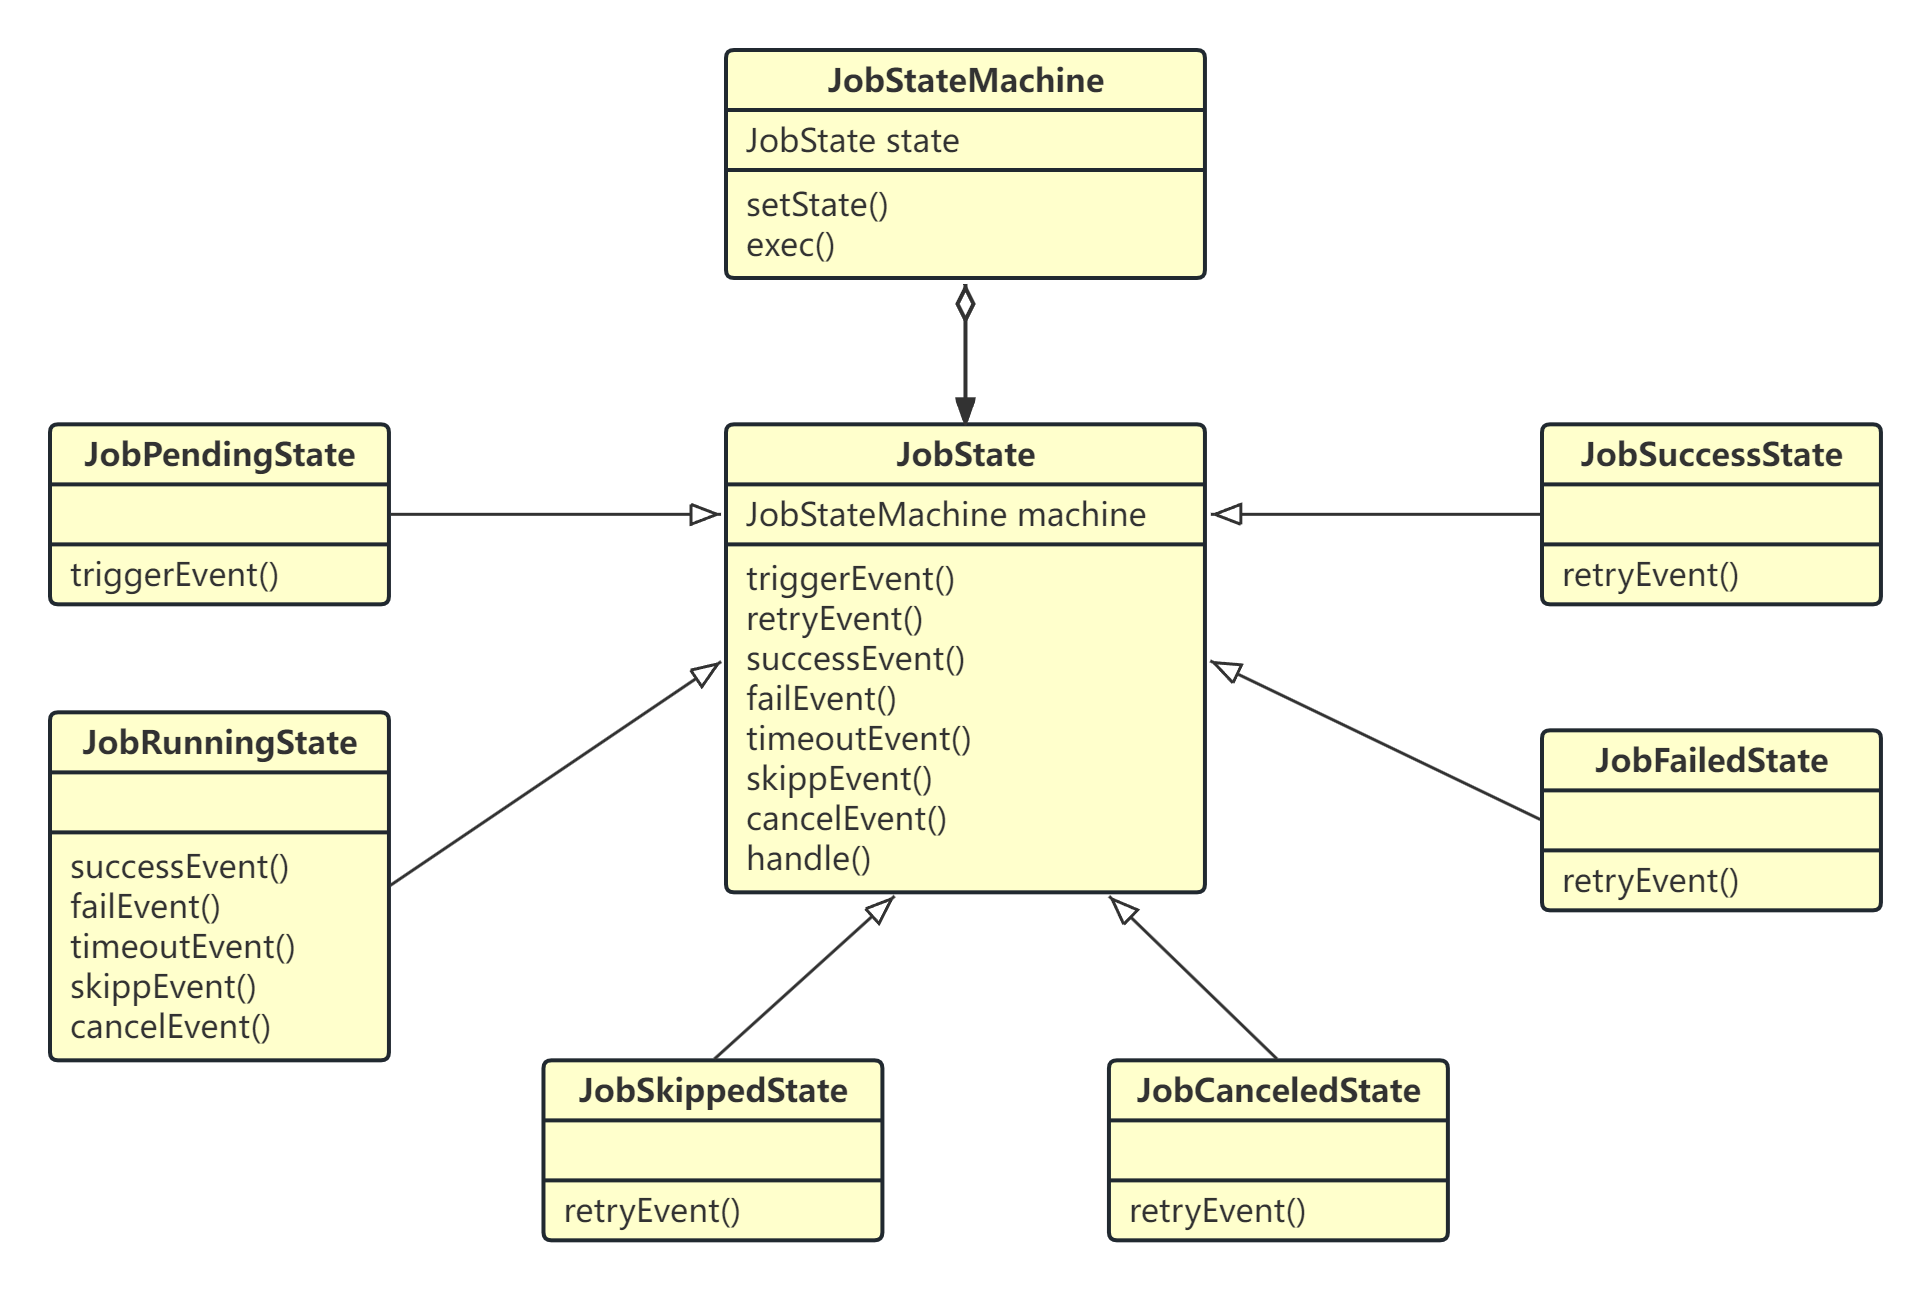
\includegraphics[width=1\textwidth]{作业状态机类图.png}
  \caption{作业状态机类图}
  \label{fig:作业状态机类图}
\end{figure}

当需要进行作业状态转换时,首先创建JobStateMachine实例并设置默认初始状态,然后向exec成员方法中传入当前发生的事件。
其中JobState是作业状态的抽象类,作业中每个具体的状态作为一个JobState的实现类,并从JobState中选择引起其状态转移的事件方法来实现。
例如JobRunningState类实现了JobState中的successEvent、failEvent、timeoutEvent、skippEvent和cancelEvent五个成员方法,这是因为这些事件均能作用于一个正在运行中的作业并且引起其状态改变,
其中successEvent方法会调用父类中持有的实例的JobStateMachine成员的setState方法,将当前状态机的状态设置为成功,并完成一些后续工作,其余事件方法也与之类似。






接下来确定状态机的事件。当一个作业运行实例被创建时其应为就绪中状态,故就绪中状态为初始状态,引发其状态改变的事件是触发(triggerEvent),
这个触发事件是由决策中心经过决策逻辑发出的,并不只是用户的动触发行为;


图~ 以作业为例实现了作业状态机。



\subsection{作业管理模块的实现}



\subsection{二级节标题}手

\subsubsection{三级节标题}

\paragraph{四级节标题}

\subparagraph{五级节标题}
